\section{Results}

\subsection{Past-Predictable Future Scenario}

\ref{tab:sim_result} lists the important metrics
obtained from the first simulation. The following
values are the EU inventory and history at year 2050.

\begin{table}[h]
	\centering
	\label{tab:sim_result}
	\caption {Simulation Results}
	\scalebox{0.86}{
		\begin{tabular}{|c|c|c|}
			\hline
			Category [unit] & Value & Specifics \\ \hline
			Total UOX Usage [t] & 188,196  &  \\ \hline
			Total MOX Usage [t] & 118 & \\ \hline
			Total Spent UOX [t] & 183,807 & \\ \hline
			Total Spent MOX [t] & 0 & All is Reprocessed. \\ \hline
			Total Tailings [t] & 1,125,798 & \\ \hline
		\end{tabular}}
\end {table}

\begin{table}[h]
	\centering
	\label{tab:pu}
	\caption{Plutonium From Spent Fuel}
	\begin{tabular}{|c|c|c|}
		\hline
		Isotope & Mass Fraction in Spent Fuel [\%] & Quantity [t] \\ \hline
		Total & .9358 & 1,761.13 \\ \hline
		Pu238 & .0111 & 20.88 \\ \
		Pu239 & .518 & 974.85 \\ \hline
		Pu240 & .232 & 436.61 \\ \hline
		Pu241 & .126 & 237.12 \\ \hline
		Pu242 & .0487 & 91.65 \\ \hline
	\end{tabular}
\end{table}


To create MOX, 10\% Pu and 90\% depleted uranium is used.
Thus $1,761.13$ tons of plutonium yields $17,611.3$ tons of
\gls{MOX}. \ref{tab:pu} lists the isotope, mass fraction,
and quantity that can be obtained from the 2050 \gls{SNF} inventory.


\subsection{French \gls{SFR} Transition Scenario}

From Varaine et al \cite{varaine_pre-conceptual_2012}, a French
ASTRID-type \gls{SFR} of capacity $600 MWe$ needs $1.225$ tons of
plutonium a year, with an initial plutonium loading of $4.9$ tons.

Thus, it can be assumed that the ASTRID reactor takes in $49$ tons of 
\gls{MOX}, and switches a quarter of its fuel every year. Simply,
an ASTRID reactor needs $12.25$ tons of \gls{MOX} per year. 

Thus the number of SFR-years worth of fuel that can be created with
the \gls{SNF} from 2050 is $\frac{17,611.3 t}{12.25} = 1,437.65 $.
Assuming infinite reprocessing and \gls{MOX} fabrication capacity,

However, assuming that \gls{MOX} can be recycled indefinitely,
spent \gls{MOX} contains enough plutonium for a \gls{MOX} fuel with
the same mass, if mixed with depleted uranium.

\begin{table}[h]
	\centering
	\label{tab:mox_waste}
	\caption{Plutonium From Spent \gls{MOX}}
	\begin{tabular}{|c|c|}
		\hline
		Isotope & Mass Fraction in Spent Fuel [\%] \\ \hline
		Total & 10.47 \\ \hline
		Pu238 & .6337 \\ \
		Pu239 & 4.302 \\ \hline
		Pu240 & 2.979 \\ \hline
		Pu241 & 1.541 \\ \hline
		Pu242 & 1.036 \\ \hline
	\end{tabular}
\end{table}

Considering that \gls{MOX} can be made from 10\% plutonium
separated from spent \gls{MOX} and 90\% depleted uranium,
\gls{MOX} can virtually be infinitely reused if there's
sufficient supply of depleted uranium and reprocessing and 
fabrication capabilities.

A simulation is run, with the tails and spent \gls{UOX}
inventory, to see if the French can transition into \gls{SFR}
without constructing additional \gls{LWR}s. An infinite
reprocessing and fabrication capacity is assumed.

\ref{fig:sfr_num} and \ref{fig:sfr_cap} displays
the \gls{SFR} number and capacity over time, as mentioned in the introduction.
The sharp increase from 2035 to 2060 is because a large number of French
reactors were built from 1975 to 2000.


\begin{figure}[htbp!]
	\begin{center}
		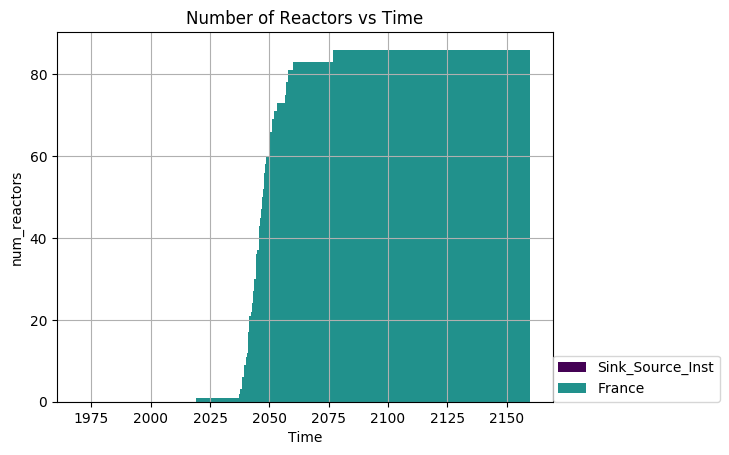
\includegraphics{./images/number_plot.png}
	\end{center}
	\caption{Timeseries of number of \gls{SFR}s}
	\label{fig:sfr_num}
\end{figure}

\begin{figure}[htbp!]
	\begin{center}
		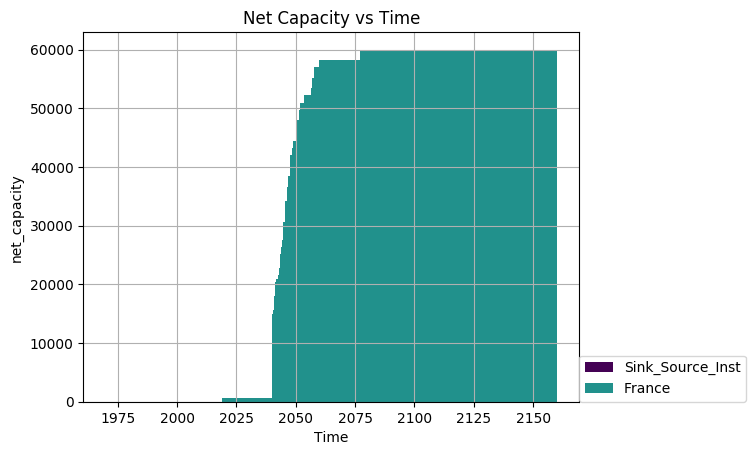
\includegraphics{./images/power_plot.png}
	\end{center}
	\caption{Timeseries of installed capacity of \gls{SFR}s}
	\label{fig:sfr_cap}
\end{figure}

\ref{fig:fuel} shows the mass of \gls{MOX} used in the 
\gls{SFR}s separated by how they are made, over time.
Note that the number of \gls{MOX} from the spent \gls{UOX}
stops increasing around 2050, which means that the spent
\gls{MOX} is enough to create the \gls{MOX} for the
\gls{SFR} fleet. 

\begin{figure}[htbp!]
	\begin{center}
		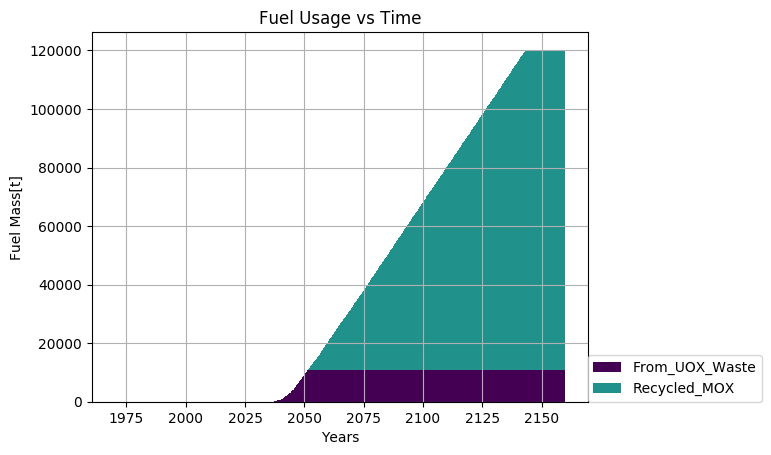
\includegraphics{./images/where_fuel.png}
	\end{center}
	\caption{Timeseries of fuel used in the \gls{SFR}s [tons]}
	\label{fig:fuel}
\end{figure}

\begin{table}[h]
	\centering
	\label{tab:sfr_sim_result}
	\caption {\gls{SFR} Simulation Results}
	\scalebox{0.86}{
		\begin{tabular}{|c|c|c|}
			\hline
			Category [unit] & Value & Specifics \\ \hline
			Total MOX used [t] & 120,261 & \\ \hline
			Total MOX from UOX Waste [t] & 10,986  &  \\ \hline
			Total MOX from MOX Waste [t] & 109,275 & \\ \hline
		\end{tabular}}
\end {table}

